\section{Projektführung}
\subsection{Rahmenplan}
\begin{figure}[H]
	\centering
	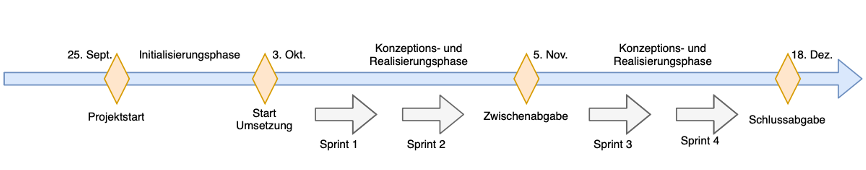
\includegraphics[width=\linewidth]{2_Projektfuehrung/Bilder/rahmenplan.png}
	\caption{Rahmenplan}
	\label{fig: Rahmenplan}
\end{figure}
Folgende Meilensteine sind gemäss Zeitstrahl zu erreichen.
\begin{center}
	\begin{tabularx}{\textwidth}{|X|X|}
		\hline
		\textbf{Meilenstein} & \textbf{Deliverable} \\
		\hline
		\textbf{Projektstart} & Beginn des Projekts, Projektteam definiert. \\
		\hline
		\textbf{Zwischenabgabe} & Rahmenplan, Projektorganisation und erste Projektrisikoliste definiert. Produktbacklog zu 80\% definiert. Sprintplanung für Sprint 1 detailliert und für Sprint 2 grob dokumentiert. \\
		\hline
		\textbf{Schlussabgabe} & Sprint 4 abgeschlossen. Nachgeführte Softwarespezifikation liegt vor und ist reviewed. Alle Komponenten sind lauffähig und demonstrierbar. Interoperabilität der Logger-Komponente ist entwickelt und demonstrierbar.. \\
		\hline
	\end{tabularx}
\end{center}
\subsection{Projektkontrolle}
\textcolor{red}{needs to be done, link zum burndownchart}
\subsection{Risikomanagement}
Folgende Auflistung zeigt die bekannten und relevanten Risiken, welche durch die Eintrittswahrscheinlichkeit und das Schadenausmass quantifiziert werden. Die Eintrittswahrscheinlichkeit wird numerisch mit einer Skala von 1 (unwahrscheinlich) bis 5 (mit grosser Wahrscheinlichkeit) dargestellt. Ebenso wird das Schadenausmass mit einer solchen Skala von 1 (harmloser Schaden) bis 5 (erheblicher Schaden) definiert.

\begin{table}[h]
	\centering
	\begin{tabular}{!{\color{black}\vrule}l!{\color{black}\vrule}l!{\color{black}\vrule}c!{\color{black}\vrule}c!{\color{black}\vrule}c!{\color{black}\vrule}} 
		\hline
		\textbf{Nr.} & \textbf{Risikobeschreibung}  & \begin{tabular}[c]{@{}c@{}} \textbf{Eintritts-}\\ \textbf{wahrscheinlichkeit} \end{tabular} & \textbf{Schadenausmass} & \begin{tabular}[c]{@{}c@{}} \textbf{Risiko} \\ \textbf{(E x S)} \end{tabular}  \\ 
		\hline
		1   & Personenausfall & 3 & 4 & 12 \\ 
		\hline
		2   & Datenverlust & 2& 5 & 10 \\ 
		\hline
		3   & Änderungen der Anforderungen & 5 & 4 & 20 \\ 
		\hline
		4   & Ausfall des Kommunikationskanals & 1 & 5 & 5 \\
		\hline
	\end{tabular}
\end{table}
\newpage
In der folgenden Tabelle werde die ergriffenen Mitigationsmassnahmen zu den oben erwähnten Risiken aufgelistet. Ebenfalls wird das Risiko neu geschätzt.
\begin{center}
		\begin{tabularx}{\linewidth}{|c|X|c|c|c|c|c|r|}
			\hline
			\multirow{2}{*}{\begin{tabular}[c]{@{}c@{}}\textbf{Risiko}\\ \textbf{Nr.}\end{tabular}} & \multirow{2}{*}{\textbf{Risikobeschreibung}} & \multicolumn{2}{c|}{\begin{tabular}[c]{@{}c@{}}\textbf{Eintritts-}\\ \textbf{wahrscheinlichkeit}\end{tabular}} & \multicolumn{2}{c|}{\textbf{Schadenausmass}} & \multicolumn{2}{c|}{\textbf{Risiko}} \\ \cline{3-8} 
			&  & \textbf{alt} & \textbf{neu} & \textbf{alt} & \textbf{neu} & \textbf{alt} & \textbf{neu} \\ \hline
			1 & E:
			Meetings via Zoom und Einhaltung der Hygienevorschriften.
			S: Sorgfältige Planung der Arbeiten, Pufferzeit einrechnen.
			 & 3 & 2 & 4 & 3 & 12 & 6 \\ \hline
			2 &E: Wahl des Speicherorts.
S: Nutzung eines Versionsverwaltungstools zur Verhinderung von Mergekonflikten
			  & 2 & 1 & 5 & 2 & 10 & 2 \\ \hline
			3 & E: kann nicht beeinflusst werden.
			S: Änderungen immer direkt im Produktbacklog festhalten und priorisieren.
			 & 5 & 5 & 4 & 2 & 20 &10  \\ \hline
			4 & E: kann nicht beeinflusst werden. 
			S: Alternative Kommunikationskanäle konfigurieren.
			 & 1 & 1 & 5 & 1 & 5 & 1 \\ \hline
		\end{tabularx}%
\end{center}

\subsection{Definition of Done}
Folgende Punkte müssen nach Vollendung eines Sprints erarbeitet sein, dass dieser als abgeschlossen definiert werden darf:
\begin{itemize}
	\item Funktionalität vollständig implementiert und integriert
	\item Unit-Tests geschrieben und durchgeführt, mit einer Testabdeckung von mindestens 70%
	\item
Funktionsfähigkeit bereits existierender Unit-Tests geprüft
	\item Keine bekannten Fehler
	\item JavaDoc vollständig
	\item Alle Änderungen wurden dokumentiert
\end{itemize}